Waste management is a constant issue, that is dealt with on the daily by different organisations.
According to Eurostat, the countries in europe have had a rather stable production of waste the past decade, while some countries fluctuate towards higher productions of waste other countries produce less. \todo{citation needed}
The above supports the claim that waste management is highly relevant in a post modern society.

However waste management has traditionally been perceived from a logistical point of view.
Imagine not the amounts nor the location of the bin being the driving force for interacting with it, but rather its smell.

This is the essential feature of our system - the additional parameter.
This additonal information can be used in conjunction with existing systems or be used to produce an entirely new experience centered around the waste bin.
Following this concept, a prototype of a simple system has been developed.
The system produces information about smell and trash level for the bin entity it is installed on.
This information is made readily available using a cloud-based system. 
We have one android application making use of the data. Its designed to be able to present in two different modes, namely as an ambient display or as an smartphone app.
Figure ~\ref{fig:smartbin} shows an overview of the system.

The system is specifically designed for private use inside a household, but can be easily adjusted and extended for different usages.

In this paper we describe the system specifications and evaluation, and discuss its potential integration in other scenarios different from the one presented.

\begin{figure}
\centering
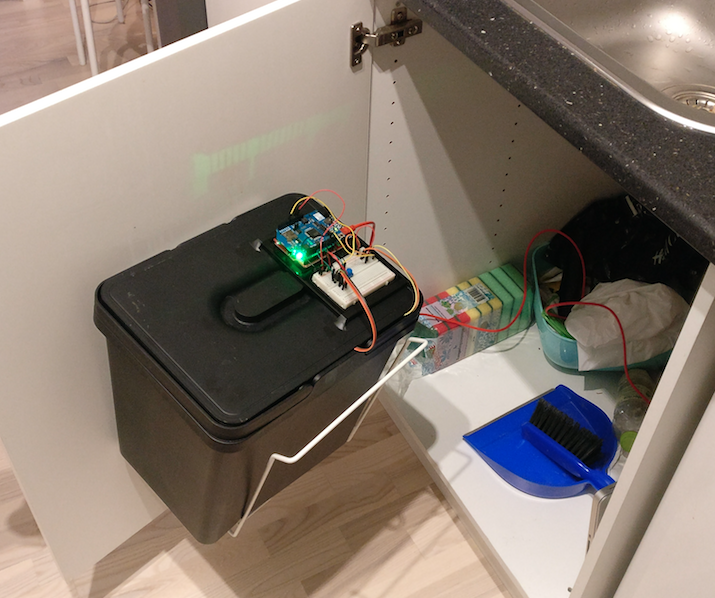
\includegraphics[scale=.2]{img/smartbin}
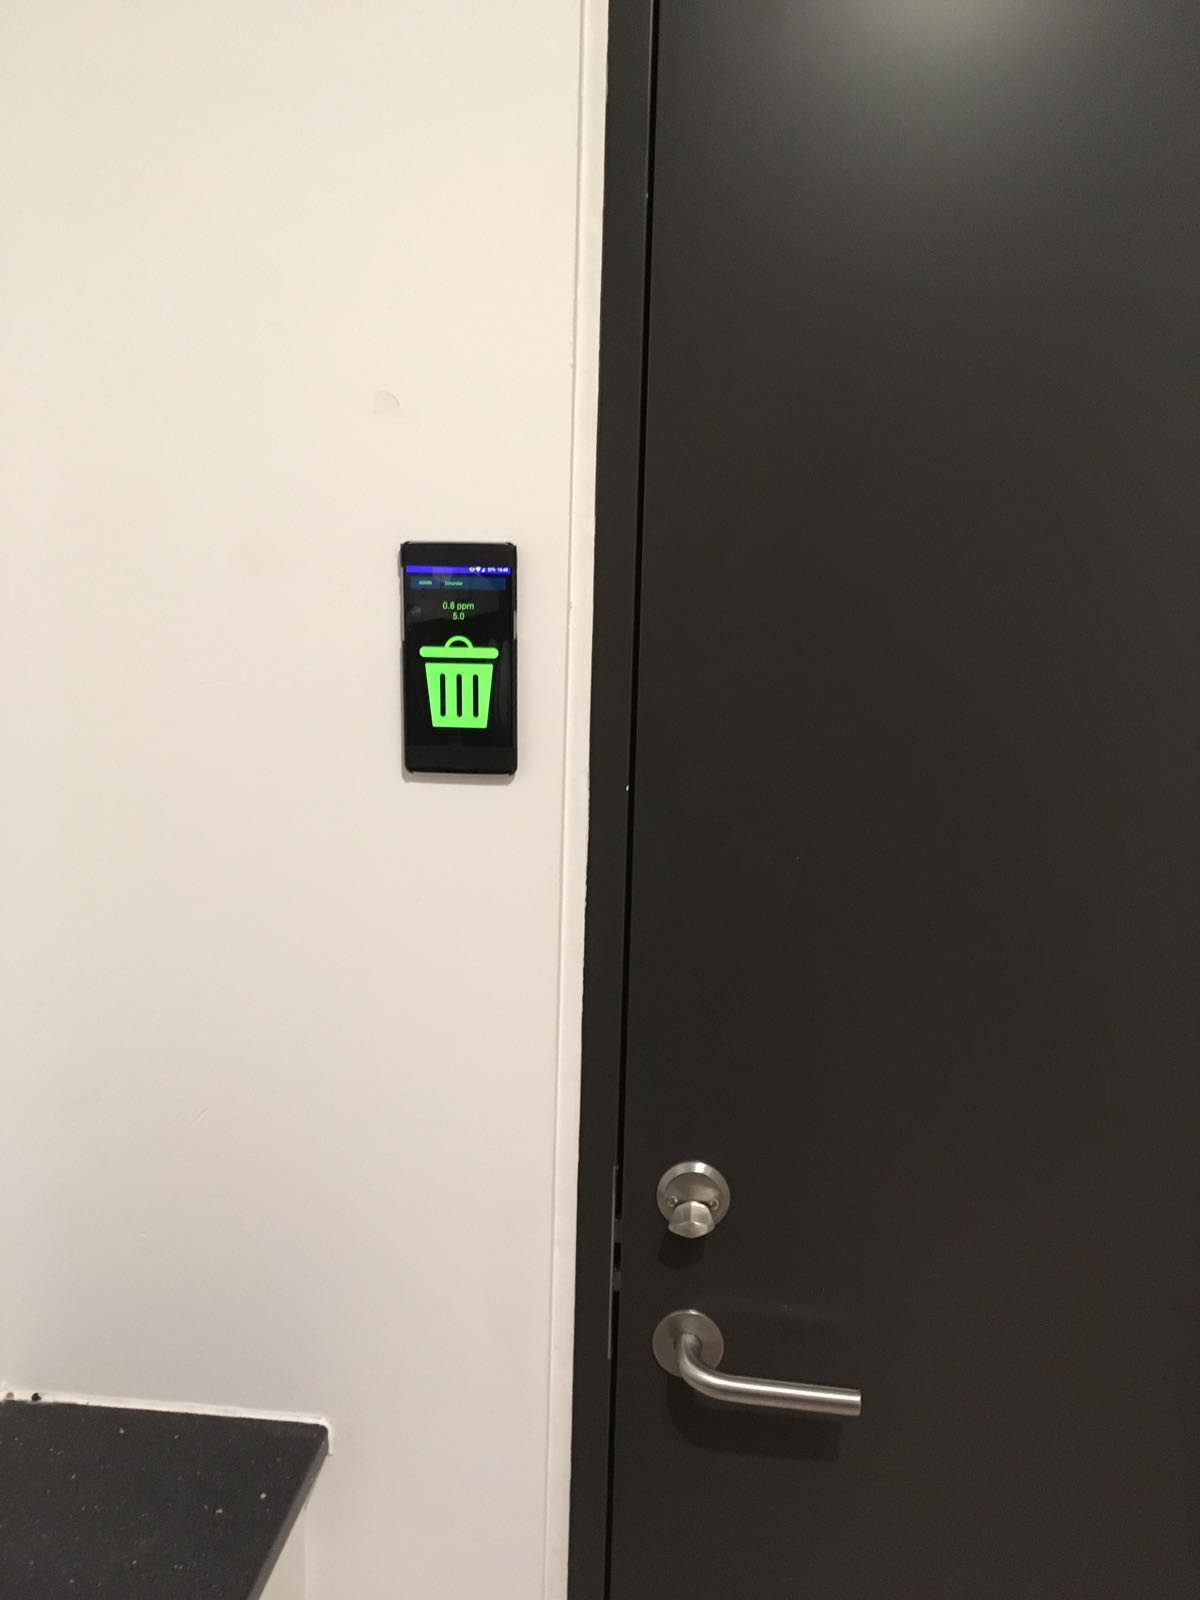
\includegraphics[scale=.075]{img/IMG-20161130-WA0000}
\caption{The SmartBin system overview, the bin with ambient display}
\label{fig:smartbin}
\end{figure}